\begin{enumerate}
\item In $\triangle ABC$ \figref{fig:Fig_2}, $AD \perp BC$. Prove that\\
$AC^2 = AB^2 + BC^2 - 2BC \times BD $
\begin{figure}[H]
    \centering
    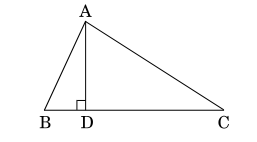
\includegraphics[width=\columnwidth]{figs/cons2.png}
    \caption{}
    \label{fig:Fig_2}
\end{figure}

\item Draw a circle of radius $4$ cm. From a point $6$ cm away from its centre, construct a pair of tangents to the circle and measure their lengths.

\item Construct a triangle with sides $5cm$, $6cm$ and $7cm$ and then another triangle whose sides are $\frac{3}{5}$ of the corresponding sides of the first triangle.

\item Let $\triangle ABC  \thicksim  \triangle DEF$  and their areas be respectively, $64cm^2$ and $121cm^2$. If $EF=15.4cm$, find $BC$.

\item Prove that the sum of the squares of the sides of a rhombus is equal to the sum of the squares of its diagonals. 

\item In \figref{fig:Fig_3}, $BL$ and $CM$ are medians of a $\triangle ABC$ right-angled at $A$. Prove that $4(BL^2 + CM^2)= 5 BC^2$. 
\begin{figure}[H]
    \centering
    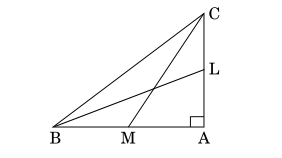
\includegraphics[width=\columnwidth]{figs/cons1.png}
    \caption{Triangle ABC}
    \label{fig:Fig_3}
\end{figure}

 \item In  \figref{fig:Fig_1}, $ABC$ is an isosceles triangle right angled at $C$ with $AC = 4 cm$. Find the length of $AB$.
\begin{figure}[H]
    \centering
    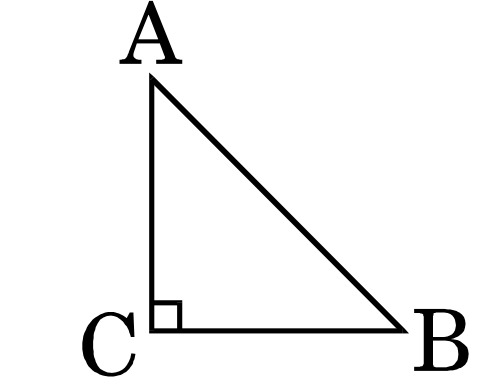
\includegraphics[width=\columnwidth]{figs/img1.jpg}
    \caption{Triangle $ABC$}
    \label{fig:Fig_1}
\end{figure}

\item In  \figref{fig:Fig_2}, $DE \parallel BC$. Find the length of side $AD$, given that $AE = 1.8 cm$, $ BD = 7.2 cm$ and $ CE = 5.4 cm$.
\begin{figure}[H]
    \centering
    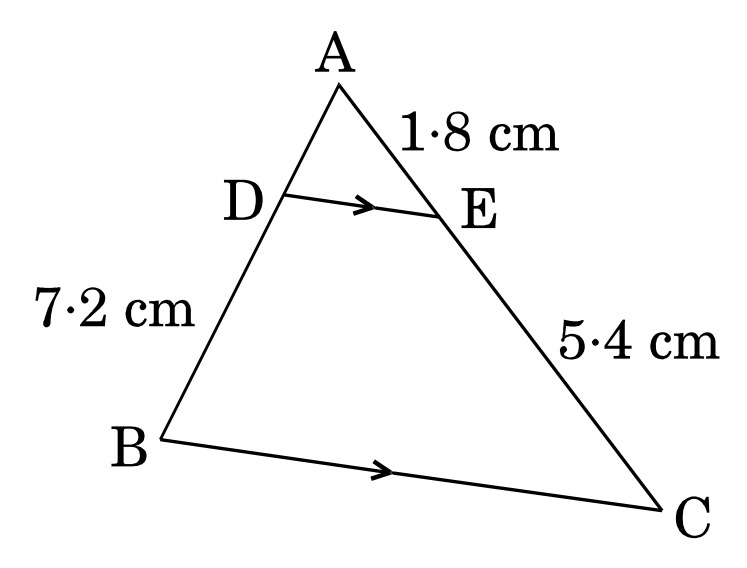
\includegraphics[width=\columnwidth]{figs/img2.jpg}
    \caption{Triangle $ABC$ }
    \label{fig:Fig_2}
\end{figure}

\item Two right triangles $ABC$ and $DBC$ are drawn on the same hypotenuse $BC$ and on the same side of $BC$. If $AC$ and $BD$ intersect at $P$, prove that $AP \times PC = BP \times DP$.

\item Construct an equilateral $\triangle ABC$ with each side $5 cm$. Then construct another triangle whose sides are $\frac{2}{3}$ times the corresponding sides of $\triangle ABC$.

\item Diagonals of a trapezium $PQRS$ intersect each other at the point $O$,
$PQ \parallel RS$ and $PQ = 3RS$. Find the ratio of the areas of triangles $POQ$ and $ROS$.
\end{enumerate}

